\documentclass[1p]{elsarticle_modified}
%\bibliographystyle{elsarticle-num}

%\usepackage[colorlinks]{hyperref}
%\usepackage{abbrmath_seonhwa} %\Abb, \Ascr, \Acal ,\Abf, \Afrak
\usepackage{amsfonts}
\usepackage{amssymb}
\usepackage{amsmath}
\usepackage{amsthm}
\usepackage{scalefnt}
\usepackage{amsbsy}
\usepackage{kotex}
\usepackage{caption}
\usepackage{subfig}
\usepackage{color}
\usepackage{graphicx}
\usepackage{xcolor} %% white, black, red, green, blue, cyan, magenta, yellow
\usepackage{float}
\usepackage{setspace}
\usepackage{hyperref}

\usepackage{tikz}
\usetikzlibrary{arrows}

\usepackage{multirow}
\usepackage{array} % fixed length table
\usepackage{hhline}

%%%%%%%%%%%%%%%%%%%%%
\makeatletter
\renewcommand*\env@matrix[1][\arraystretch]{%
	\edef\arraystretch{#1}%
	\hskip -\arraycolsep
	\let\@ifnextchar\new@ifnextchar
	\array{*\c@MaxMatrixCols c}}
\makeatother %https://tex.stackexchange.com/questions/14071/how-can-i-increase-the-line-spacing-in-a-matrix
%%%%%%%%%%%%%%%

\usepackage[normalem]{ulem}

\newcommand{\msout}[1]{\ifmmode\text{\sout{\ensuremath{#1}}}\else\sout{#1}\fi}
%SOURCE: \msout is \stkout macro in https://tex.stackexchange.com/questions/20609/strikeout-in-math-mode

\newcommand{\cancel}[1]{
	\ifmmode
	{\color{red}\msout{#1}}
	\else
	{\color{red}\sout{#1}}
	\fi
}

\newcommand{\add}[1]{
	{\color{blue}\uwave{#1}}
}

\newcommand{\replace}[2]{
	\ifmmode
	{\color{red}\msout{#1}}{\color{blue}\uwave{#2}}
	\else
	{\color{red}\sout{#1}}{\color{blue}\uwave{#2}}
	\fi
}

\newcommand{\Sol}{\mathcal{S}} %segment
\newcommand{\D}{D} %diagram
\newcommand{\A}{\mathcal{A}} %arc


%%%%%%%%%%%%%%%%%%%%%%%%%%%%%5 test

\def\sl{\operatorname{\textup{SL}}(2,\Cbb)}
\def\psl{\operatorname{\textup{PSL}}(2,\Cbb)}
\def\quan{\mkern 1mu \triangleright \mkern 1mu}

\theoremstyle{definition}
\newtheorem{thm}{Theorem}[section]
\newtheorem{prop}[thm]{Proposition}
\newtheorem{lem}[thm]{Lemma}
\newtheorem{ques}[thm]{Question}
\newtheorem{cor}[thm]{Corollary}
\newtheorem{defn}[thm]{Definition}
\newtheorem{exam}[thm]{Example}
\newtheorem{rmk}[thm]{Remark}
\newtheorem{alg}[thm]{Algorithm}

\newcommand{\I}{\sqrt{-1}}
\begin{document}

%\begin{frontmatter}
%
%\title{Boundary parabolic representations of knots up to 8 crossings}
%
%%% Group authors per affiliation:
%\author{Yunhi Cho} 
%\address{Department of Mathematics, University of Seoul, Seoul, Korea}
%\ead{yhcho@uos.ac.kr}
%
%
%\author{Seonhwa Kim} %\fnref{s_kim}}
%\address{Center for Geometry and Physics, Institute for Basic Science, Pohang, 37673, Korea}
%\ead{ryeona17@ibs.re.kr}
%
%\author{Hyuk Kim}
%\address{Department of Mathematical Sciences, Seoul National University, Seoul 08826, Korea}
%\ead{hyukkim@snu.ac.kr}
%
%\author{Seokbeom Yoon}
%\address{Department of Mathematical Sciences, Seoul National University, Seoul, 08826,  Korea}
%\ead{sbyoon15@snu.ac.kr}
%
%\begin{abstract}
%We find all boundary parabolic representation of knots up to 8 crossings.
%
%\end{abstract}
%\begin{keyword}
%    \MSC[2010] 57M25 
%\end{keyword}
%
%\end{frontmatter}

%\linenumbers
%\tableofcontents
%
\newcommand\colored[1]{\textcolor{white}{\rule[-0.35ex]{0.8em}{1.4ex}}\kern-0.8em\color{red} #1}%
%\newcommand\colored[1]{\textcolor{white}{ #1}\kern-2.17ex	\textcolor{white}{ #1}\kern-1.81ex	\textcolor{white}{ #1}\kern-2.15ex\color{red}#1	}

{\Large $\underline{12a_{0908}~(K12a_{0908})}$}

\setlength{\tabcolsep}{10pt}
\renewcommand{\arraystretch}{1.6}
\vspace{1cm}\begin{tabular}{m{100pt}>{\centering\arraybackslash}m{274pt}}
\multirow{5}{120pt}{
	\centering
	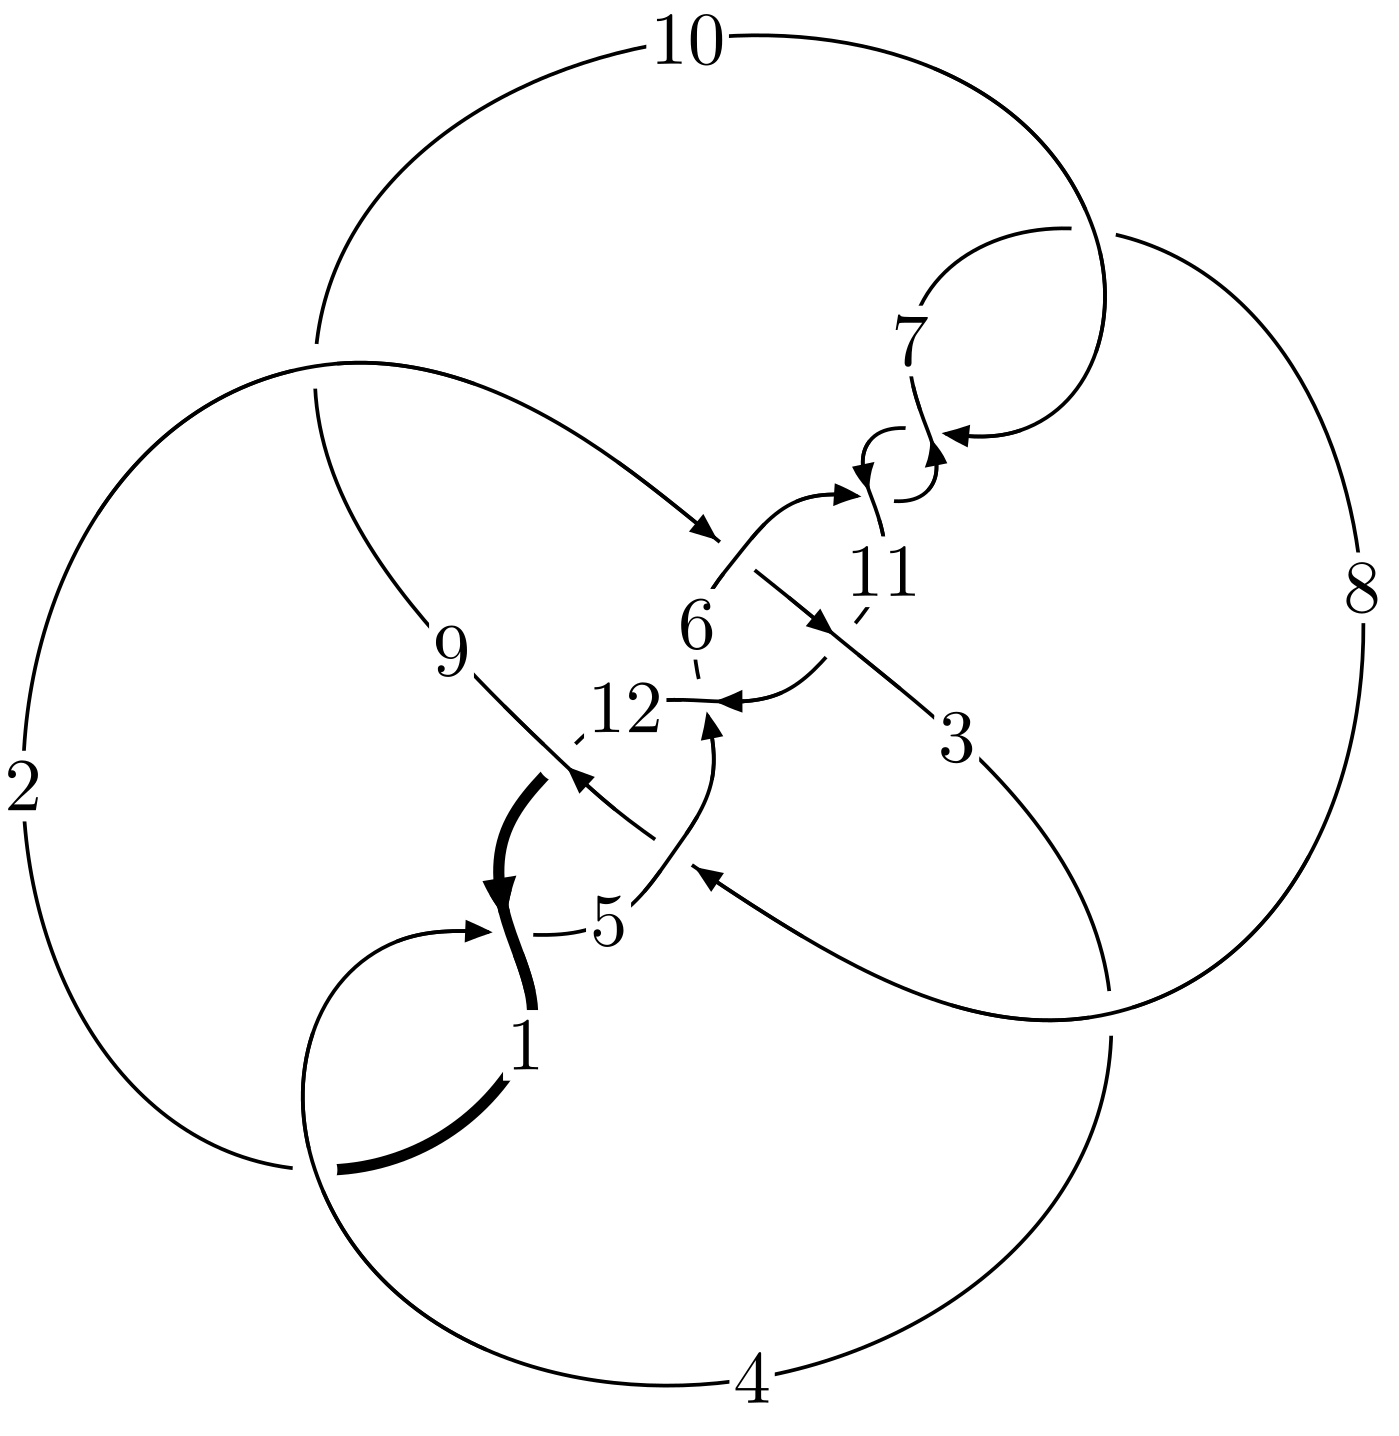
\includegraphics[width=112pt]{../../../GIT/diagram.site/Diagrams/png/1709_12a_0908.png}\\
\ \ \ A knot diagram\footnotemark}&
\allowdisplaybreaks
\textbf{Linearized knot diagam} \\
\cline{2-2}
 &
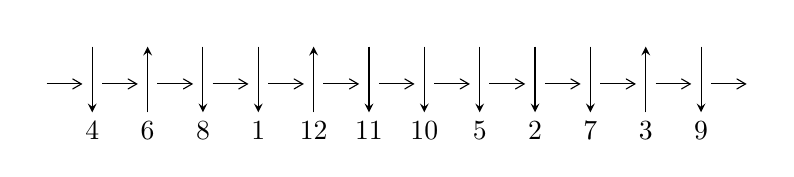
\begin{tikzpicture}[x=20pt, y=17pt]
	% nodes
	\node (C0) at (0, 0) {};
	\node (C1) at (1, 0) {};
	\node (C1U) at (1, +1) {};
	\node (C1D) at (1, -1) {4};

	\node (C2) at (2, 0) {};
	\node (C2U) at (2, +1) {};
	\node (C2D) at (2, -1) {6};

	\node (C3) at (3, 0) {};
	\node (C3U) at (3, +1) {};
	\node (C3D) at (3, -1) {8};

	\node (C4) at (4, 0) {};
	\node (C4U) at (4, +1) {};
	\node (C4D) at (4, -1) {1};

	\node (C5) at (5, 0) {};
	\node (C5U) at (5, +1) {};
	\node (C5D) at (5, -1) {12};

	\node (C6) at (6, 0) {};
	\node (C6U) at (6, +1) {};
	\node (C6D) at (6, -1) {11};

	\node (C7) at (7, 0) {};
	\node (C7U) at (7, +1) {};
	\node (C7D) at (7, -1) {10};

	\node (C8) at (8, 0) {};
	\node (C8U) at (8, +1) {};
	\node (C8D) at (8, -1) {5};

	\node (C9) at (9, 0) {};
	\node (C9U) at (9, +1) {};
	\node (C9D) at (9, -1) {2};

	\node (C10) at (10, 0) {};
	\node (C10U) at (10, +1) {};
	\node (C10D) at (10, -1) {7};

	\node (C11) at (11, 0) {};
	\node (C11U) at (11, +1) {};
	\node (C11D) at (11, -1) {3};

	\node (C12) at (12, 0) {};
	\node (C12U) at (12, +1) {};
	\node (C12D) at (12, -1) {9};
	\node (C13) at (13, 0) {};

	% arrows
	\draw[->,>={angle 60}]
	(C0) edge (C1) (C1) edge (C2) (C2) edge (C3) (C3) edge (C4) (C4) edge (C5) (C5) edge (C6) (C6) edge (C7) (C7) edge (C8) (C8) edge (C9) (C9) edge (C10) (C10) edge (C11) (C11) edge (C12) (C12) edge (C13) ;	\draw[->,>=stealth]
	(C1U) edge (C1D) (C2D) edge (C2U) (C3U) edge (C3D) (C4U) edge (C4D) (C5D) edge (C5U) (C6U) edge (C6D) (C7U) edge (C7D) (C8U) edge (C8D) (C9U) edge (C9D) (C10U) edge (C10D) (C11D) edge (C11U) (C12U) edge (C12D) ;
	\end{tikzpicture} \\
\hhline{~~} \\& 
\textbf{Solving Sequence} \\ \cline{2-2} 
 &
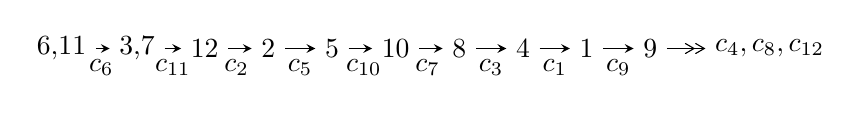
\begin{tikzpicture}[x=23pt, y=7pt]
	% node
	\node (A0) at (-1/8, 0) {6,11};
	\node (A1) at (17/16, 0) {3,7};
	\node (A2) at (17/8, 0) {12};
	\node (A3) at (25/8, 0) {2};
	\node (A4) at (33/8, 0) {5};
	\node (A5) at (41/8, 0) {10};
	\node (A6) at (49/8, 0) {8};
	\node (A7) at (57/8, 0) {4};
	\node (A8) at (65/8, 0) {1};
	\node (A9) at (73/8, 0) {9};
	\node (C1) at (1/2, -1) {$c_{6}$};
	\node (C2) at (13/8, -1) {$c_{11}$};
	\node (C3) at (21/8, -1) {$c_{2}$};
	\node (C4) at (29/8, -1) {$c_{5}$};
	\node (C5) at (37/8, -1) {$c_{10}$};
	\node (C6) at (45/8, -1) {$c_{7}$};
	\node (C7) at (53/8, -1) {$c_{3}$};
	\node (C8) at (61/8, -1) {$c_{1}$};
	\node (C9) at (69/8, -1) {$c_{9}$};
	\node (A10) at (11, 0) {$c_{4},c_{8},c_{12}$};

	% edge
	\draw[->,>=stealth]	
	(A0) edge (A1) (A1) edge (A2) (A2) edge (A3) (A3) edge (A4) (A4) edge (A5) (A5) edge (A6) (A6) edge (A7) (A7) edge (A8) (A8) edge (A9) ;
	\draw[->>,>={angle 60}]	
	(A9) edge (A10);
\end{tikzpicture} \\ 

\end{tabular} \\

\footnotetext{
The image of knot diagram is generated by the software ``\textbf{Draw programme}" developed by Andrew Bartholomew(\url{http://www.layer8.co.uk/maths/draw/index.htm\#Running-draw}), where we modified some parts for our purpose(\url{https://github.com/CATsTAILs/LinksPainter}).
}\phantom \\ \newline 
\centering \textbf{Ideals for irreducible components\footnotemark of $X_{\text{par}}$} 
 
\begin{align*}
I^u_{1}&=\langle 
-8.64139\times10^{24} u^{52}-1.07961\times10^{26} u^{51}+\cdots+7.39787\times10^{23} b+6.82500\times10^{25},\\
\phantom{I^u_{1}}&\phantom{= \langle  }-3.41250\times10^{25} u^{52}-4.26342\times10^{26} u^{51}+\cdots+1.47957\times10^{24} a+2.88944\times10^{26},\\
\phantom{I^u_{1}}&\phantom{= \langle  }u^{53}+13 u^{52}+\cdots-18 u-4\rangle \\
I^u_{2}&=\langle 
56634753 u^{22} a^3-240804262 u^{22} a^2+\cdots-330550633 a-132611191,\\
\phantom{I^u_{2}}&\phantom{= \langle  }- u^{22} a^3+5 u^{22} a^2+\cdots-4 a+51,\;u^{23}-5 u^{22}+\cdots-6 u^2+1\rangle \\
I^u_{3}&=\langle 
59 u^{27}-471 u^{26}+\cdots+47 b-50,\;50 u^{27}-341 u^{26}+\cdots+47 a+58,\;u^{28}-8 u^{27}+\cdots-2 u+1\rangle \\
\\
\end{align*}
\raggedright * 3 irreducible components of $\dim_{\mathbb{C}}=0$, with total 173 representations.\\
\footnotetext{All coefficients of polynomials are rational numbers. But the coefficients are sometimes approximated in decimal forms when there is not enough margin.}
\newpage
\renewcommand{\arraystretch}{1}
\centering \section*{I. $I^u_{1}= \langle -8.64\times10^{24} u^{52}-1.08\times10^{26} u^{51}+\cdots+7.40\times10^{23} b+6.83\times10^{25},\;-3.41\times10^{25} u^{52}-4.26\times10^{26} u^{51}+\cdots+1.48\times10^{24} a+2.89\times10^{26},\;u^{53}+13 u^{52}+\cdots-18 u-4 \rangle$}
\flushleft \textbf{(i) Arc colorings}\\
\begin{tabular}{m{7pt} m{180pt} m{7pt} m{180pt} }
\flushright $a_{6}=$&$\begin{pmatrix}1\\0\end{pmatrix}$ \\
\flushright $a_{11}=$&$\begin{pmatrix}0\\u\end{pmatrix}$ \\
\flushright $a_{3}=$&$\begin{pmatrix}23.0641 u^{52}+288.152 u^{51}+\cdots-461.727 u-195.289\\11.6809 u^{52}+145.935 u^{51}+\cdots-219.864 u-92.2563\end{pmatrix}$ \\
\flushright $a_{7}=$&$\begin{pmatrix}1\\u^2\end{pmatrix}$ \\
\flushright $a_{12}=$&$\begin{pmatrix}34.8240 u^{52}+435.869 u^{51}+\cdots-659.197 u-297.311\\16.8427 u^{52}+210.735 u^{51}+\cdots-328.520 u-139.296\end{pmatrix}$ \\
\flushright $a_{2}=$&$\begin{pmatrix}11.3832 u^{52}+142.217 u^{51}+\cdots-241.863 u-103.033\\11.6809 u^{52}+145.935 u^{51}+\cdots-219.864 u-92.2563\end{pmatrix}$ \\
\flushright $a_{5}=$&$\begin{pmatrix}-38.2045 u^{52}-480.262 u^{51}+\cdots+774.344 u+369.617\\-24.6163 u^{52}-310.110 u^{51}+\cdots+482.937 u+220.189\end{pmatrix}$ \\
\flushright $a_{10}=$&$\begin{pmatrix}u\\u^3+u\end{pmatrix}$ \\
\flushright $a_{8}=$&$\begin{pmatrix}u^2+1\\u^4+2 u^2\end{pmatrix}$ \\
\flushright $a_{4}=$&$\begin{pmatrix}21.0832 u^{52}+263.927 u^{51}+\cdots-431.740 u-179.708\\9.66738 u^{52}+121.370 u^{51}+\cdots-192.750 u-83.0710\end{pmatrix}$ \\
\flushright $a_{1}=$&$\begin{pmatrix}40.8118 u^{52}+510.563 u^{51}+\cdots-813.034 u-355.160\\25.5389 u^{52}+319.906 u^{51}+\cdots-495.955 u-211.836\end{pmatrix}$ \\
\flushright $a_{9}=$&$\begin{pmatrix}3.42379 u^{52}+43.8595 u^{51}+\cdots-53.5420 u-34.9635\\1.13831 u^{52}+14.3096 u^{51}+\cdots-27.9059 u-18.2484\end{pmatrix}$\\&\end{tabular}
\flushleft \textbf{(ii) Obstruction class $= -1$}\\~\\
\flushleft \textbf{(iii) Cusp Shapes $= \frac{7813885398705379548002022}{369893658631687521362639} u^{52}+\frac{97738403535384698831973970}{369893658631687521362639} u^{51}+\cdots-\frac{144011829016585325244113120}{369893658631687521362639} u-\frac{67086585797972419521829478}{369893658631687521362639}$}\\~\\
\newpage\renewcommand{\arraystretch}{1}
\flushleft \textbf{(iv) u-Polynomials at the component}\newline \\
\begin{tabular}{m{50pt}|m{274pt}}
Crossings & \hspace{64pt}u-Polynomials at each crossing \\
\hline $$\begin{aligned}c_{1},c_{4}\end{aligned}$$&$\begin{aligned}
&u^{53}-21 u^{52}+\cdots-3256 u+192
\end{aligned}$\\
\hline $$\begin{aligned}c_{2},c_{11}\end{aligned}$$&$\begin{aligned}
&u^{53}-3 u^{52}+\cdots+7 u+1
\end{aligned}$\\
\hline $$\begin{aligned}c_{3},c_{9}\end{aligned}$$&$\begin{aligned}
&u^{53}- u^{52}+\cdots-12 u+1
\end{aligned}$\\
\hline $$\begin{aligned}c_{5}\end{aligned}$$&$\begin{aligned}
&u^{53}-38 u^{52}+\cdots-150994944 u+8388608
\end{aligned}$\\
\hline $$\begin{aligned}c_{6},c_{7},c_{10}\end{aligned}$$&$\begin{aligned}
&u^{53}-13 u^{52}+\cdots-18 u+4
\end{aligned}$\\
\hline $$\begin{aligned}c_{8},c_{12}\end{aligned}$$&$\begin{aligned}
&u^{53}+u^{52}+\cdots+18 u^2+1
\end{aligned}$\\
\hline
\end{tabular}\\~\\
\newpage\renewcommand{\arraystretch}{1}
\flushleft \textbf{(v) Riley Polynomials at the component}\newline \\
\begin{tabular}{m{50pt}|m{274pt}}
Crossings & \hspace{64pt}Riley Polynomials at each crossing \\
\hline $$\begin{aligned}c_{1},c_{4}\end{aligned}$$&$\begin{aligned}
&y^{53}+39 y^{52}+\cdots+230080 y-36864
\end{aligned}$\\
\hline $$\begin{aligned}c_{2},c_{11}\end{aligned}$$&$\begin{aligned}
&y^{53}-25 y^{52}+\cdots-89 y-1
\end{aligned}$\\
\hline $$\begin{aligned}c_{3},c_{9}\end{aligned}$$&$\begin{aligned}
&y^{53}-5 y^{52}+\cdots+10 y-1
\end{aligned}$\\
\hline $$\begin{aligned}c_{5}\end{aligned}$$&$\begin{aligned}
&y^{53}+16 y^{52}+\cdots+140737488355328 y-70368744177664
\end{aligned}$\\
\hline $$\begin{aligned}c_{6},c_{7},c_{10}\end{aligned}$$&$\begin{aligned}
&y^{53}+51 y^{52}+\cdots+764 y-16
\end{aligned}$\\
\hline $$\begin{aligned}c_{8},c_{12}\end{aligned}$$&$\begin{aligned}
&y^{53}+17 y^{52}+\cdots-36 y-1
\end{aligned}$\\
\hline
\end{tabular}\\~\\
\newpage\flushleft \textbf{(vi) Complex Volumes and Cusp Shapes}
$$\begin{array}{c|c|c}  
\text{Solutions to }I^u_{1}& \I (\text{vol} + \sqrt{-1}CS) & \text{Cusp shape}\\
 \hline 
\begin{aligned}
u &= -0.705381 + 0.706977 I \\
a &= \phantom{-}0.940947 + 0.011228 I \\
b &= \phantom{-}0.671664 - 0.657308 I\end{aligned}
 & -3.12391 - 4.65185 I & \phantom{-0.000000 } 0 \\ \hline\begin{aligned}
u &= -0.705381 - 0.706977 I \\
a &= \phantom{-}0.940947 - 0.011228 I \\
b &= \phantom{-}0.671664 + 0.657308 I\end{aligned}
 & -3.12391 + 4.65185 I & \phantom{-0.000000 } 0 \\ \hline\begin{aligned}
u &= -0.846780 + 0.538162 I \\
a &= -0.299959 - 1.372480 I \\
b &= -0.992613 - 1.000760 I\end{aligned}
 & -0.0493 + 15.5803 I & \phantom{-0.000000 } 0 \\ \hline\begin{aligned}
u &= -0.846780 - 0.538162 I \\
a &= -0.299959 + 1.372480 I \\
b &= -0.992613 + 1.000760 I\end{aligned}
 & -0.0493 - 15.5803 I & \phantom{-0.000000 } 0 \\ \hline\begin{aligned}
u &= -0.921335 + 0.403223 I \\
a &= \phantom{-}0.731872 + 0.584881 I \\
b &= \phantom{-}0.910136 + 0.243764 I\end{aligned}
 & \phantom{-}4.18006 + 7.18781 I & \phantom{-0.000000 } 0 \\ \hline\begin{aligned}
u &= -0.921335 - 0.403223 I \\
a &= \phantom{-}0.731872 - 0.584881 I \\
b &= \phantom{-}0.910136 - 0.243764 I\end{aligned}
 & \phantom{-}4.18006 - 7.18781 I & \phantom{-0.000000 } 0 \\ \hline\begin{aligned}
u &= -0.537871 + 0.784035 I \\
a &= \phantom{-}0.278841 + 0.943890 I \\
b &= \phantom{-}0.890023 + 0.289070 I\end{aligned}
 & \phantom{-}5.74699 - 1.95135 I & \phantom{-0.000000 } 0 \\ \hline\begin{aligned}
u &= -0.537871 - 0.784035 I \\
a &= \phantom{-}0.278841 - 0.943890 I \\
b &= \phantom{-}0.890023 - 0.289070 I\end{aligned}
 & \phantom{-}5.74699 + 1.95135 I & \phantom{-0.000000 } 0 \\ \hline\begin{aligned}
u &= -0.795408 + 0.442380 I \\
a &= \phantom{-}0.43381 + 1.47445 I \\
b &= \phantom{-}0.997322 + 0.980880 I\end{aligned}
 & -3.88201 + 9.72876 I & \phantom{-0.000000 } 0 \\ \hline\begin{aligned}
u &= -0.795408 - 0.442380 I \\
a &= \phantom{-}0.43381 - 1.47445 I \\
b &= \phantom{-}0.997322 - 0.980880 I\end{aligned}
 & -3.88201 - 9.72876 I & \phantom{-0.000000 } 0\\
 \hline 
 \end{array}$$\newpage$$\begin{array}{c|c|c}  
\text{Solutions to }I^u_{1}& \I (\text{vol} + \sqrt{-1}CS) & \text{Cusp shape}\\
 \hline 
\begin{aligned}
u &= -0.884649 + 0.636725 I \\
a &= -0.861899 + 0.160096 I \\
b &= -0.660540 + 0.690422 I\end{aligned}
 & \phantom{-}0.16418 - 9.89272 I & \phantom{-0.000000 } 0 \\ \hline\begin{aligned}
u &= -0.884649 - 0.636725 I \\
a &= -0.861899 - 0.160096 I \\
b &= -0.660540 - 0.690422 I\end{aligned}
 & \phantom{-}0.16418 + 9.89272 I & \phantom{-0.000000 } 0 \\ \hline\begin{aligned}
u &= \phantom{-}1.166540 + 0.234114 I \\
a &= -0.0096401 + 0.0930633 I \\
b &= \phantom{-}0.0330331 - 0.1063050 I\end{aligned}
 & -1.01570 - 1.08166 I & \phantom{-0.000000 } 0 \\ \hline\begin{aligned}
u &= \phantom{-}1.166540 - 0.234114 I \\
a &= -0.0096401 - 0.0930633 I \\
b &= \phantom{-}0.0330331 + 0.1063050 I\end{aligned}
 & -1.01570 + 1.08166 I & \phantom{-0.000000 } 0 \\ \hline\begin{aligned}
u &= \phantom{-}0.132150 + 1.227450 I \\
a &= -0.614846 + 0.058087 I \\
b &= \phantom{-}0.152551 + 0.747014 I\end{aligned}
 & \phantom{-}2.82416 - 2.70237 I & \phantom{-0.000000 } 0 \\ \hline\begin{aligned}
u &= \phantom{-}0.132150 - 1.227450 I \\
a &= -0.614846 - 0.058087 I \\
b &= \phantom{-}0.152551 - 0.747014 I\end{aligned}
 & \phantom{-}2.82416 + 2.70237 I & \phantom{-0.000000 } 0 \\ \hline\begin{aligned}
u &= -0.056333 + 1.254440 I \\
a &= -0.168258 + 0.728529 I \\
b &= \phantom{-}0.904418 + 0.252110 I\end{aligned}
 & \phantom{-}5.40952 - 2.59372 I & \phantom{-0.000000 } 0 \\ \hline\begin{aligned}
u &= -0.056333 - 1.254440 I \\
a &= -0.168258 - 0.728529 I \\
b &= \phantom{-}0.904418 - 0.252110 I\end{aligned}
 & \phantom{-}5.40952 + 2.59372 I & \phantom{-0.000000 } 0 \\ \hline\begin{aligned}
u &= -0.586615 + 0.265441 I \\
a &= -1.03974 - 1.14731 I \\
b &= -0.914471 - 0.397042 I\end{aligned}
 & \phantom{-}1.49476 + 1.54837 I & \phantom{-}1.89519 - 3.54470 I \\ \hline\begin{aligned}
u &= -0.586615 - 0.265441 I \\
a &= -1.03974 + 1.14731 I \\
b &= -0.914471 + 0.397042 I\end{aligned}
 & \phantom{-}1.49476 - 1.54837 I & \phantom{-}1.89519 + 3.54470 I\\
 \hline 
 \end{array}$$\newpage$$\begin{array}{c|c|c}  
\text{Solutions to }I^u_{1}& \I (\text{vol} + \sqrt{-1}CS) & \text{Cusp shape}\\
 \hline 
\begin{aligned}
u &= -0.521207 + 0.343252 I \\
a &= -0.40504 - 2.22925 I \\
b &= -0.976303 - 1.022870 I\end{aligned}
 & \phantom{-}1.59267 + 3.97075 I & \phantom{-}8.04998 - 10.15076 I \\ \hline\begin{aligned}
u &= -0.521207 - 0.343252 I \\
a &= -0.40504 + 2.22925 I \\
b &= -0.976303 + 1.022870 I\end{aligned}
 & \phantom{-}1.59267 - 3.97075 I & \phantom{-}8.04998 + 10.15076 I \\ \hline\begin{aligned}
u &= -0.041141 + 1.384110 I \\
a &= \phantom{-}0.621792 - 0.871465 I \\
b &= -1.18062 - 0.89648 I\end{aligned}
 & \phantom{-}5.84394 + 2.71782 I & \phantom{-0.000000 } 0 \\ \hline\begin{aligned}
u &= -0.041141 - 1.384110 I \\
a &= \phantom{-}0.621792 + 0.871465 I \\
b &= -1.18062 + 0.89648 I\end{aligned}
 & \phantom{-}5.84394 - 2.71782 I & \phantom{-0.000000 } 0 \\ \hline\begin{aligned}
u &= \phantom{-}0.04414 + 1.42109 I \\
a &= -0.703415 + 0.845262 I \\
b &= \phantom{-}1.23224 + 0.96230 I\end{aligned}
 & \phantom{-}6.72507 + 1.35266 I & \phantom{-0.000000 } 0 \\ \hline\begin{aligned}
u &= \phantom{-}0.04414 - 1.42109 I \\
a &= -0.703415 - 0.845262 I \\
b &= \phantom{-}1.23224 - 0.96230 I\end{aligned}
 & \phantom{-}6.72507 - 1.35266 I & \phantom{-0.000000 } 0 \\ \hline\begin{aligned}
u &= -0.36334 + 1.37838 I \\
a &= -0.221898 - 0.637733 I \\
b &= -0.959664 + 0.074146 I\end{aligned}
 & \phantom{-}5.57512 + 2.07297 I & \phantom{-0.000000 } 0 \\ \hline\begin{aligned}
u &= -0.36334 - 1.37838 I \\
a &= -0.221898 + 0.637733 I \\
b &= -0.959664 - 0.074146 I\end{aligned}
 & \phantom{-}5.57512 - 2.07297 I & \phantom{-0.000000 } 0 \\ \hline\begin{aligned}
u &= \phantom{-}0.08011 + 1.44842 I \\
a &= \phantom{-}0.388708 - 0.632540 I \\
b &= -0.947321 - 0.512342 I\end{aligned}
 & \phantom{-}7.93090 - 3.01833 I & \phantom{-0.000000 } 0 \\ \hline\begin{aligned}
u &= \phantom{-}0.08011 - 1.44842 I \\
a &= \phantom{-}0.388708 + 0.632540 I \\
b &= -0.947321 + 0.512342 I\end{aligned}
 & \phantom{-}7.93090 + 3.01833 I & \phantom{-0.000000 } 0\\
 \hline 
 \end{array}$$\newpage$$\begin{array}{c|c|c}  
\text{Solutions to }I^u_{1}& \I (\text{vol} + \sqrt{-1}CS) & \text{Cusp shape}\\
 \hline 
\begin{aligned}
u &= -0.19568 + 1.44259 I \\
a &= \phantom{-}0.702045 - 1.064010 I \\
b &= -1.39755 - 1.22097 I\end{aligned}
 & \phantom{-}7.37959 + 6.62771 I & \phantom{-0.000000 } 0 \\ \hline\begin{aligned}
u &= -0.19568 - 1.44259 I \\
a &= \phantom{-}0.702045 + 1.064010 I \\
b &= -1.39755 + 1.22097 I\end{aligned}
 & \phantom{-}7.37959 - 6.62771 I & \phantom{-0.000000 } 0 \\ \hline\begin{aligned}
u &= \phantom{-}0.536362\phantom{ +0.000000I} \\
a &= -0.412615\phantom{ +0.000000I} \\
b &= \phantom{-}0.221311\phantom{ +0.000000I}\end{aligned}
 & -0.915843\phantom{ +0.000000I} & -11.2030\phantom{ +0.000000I} \\ \hline\begin{aligned}
u &= -0.24997 + 1.44388 I \\
a &= \phantom{-}0.287466 - 1.002230 I \\
b &= -1.37525 - 0.66560 I\end{aligned}
 & \phantom{-}7.08466 + 4.78253 I & \phantom{-0.000000 } 0 \\ \hline\begin{aligned}
u &= -0.24997 - 1.44388 I \\
a &= \phantom{-}0.287466 + 1.002230 I \\
b &= -1.37525 + 0.66560 I\end{aligned}
 & \phantom{-}7.08466 - 4.78253 I & \phantom{-0.000000 } 0 \\ \hline\begin{aligned}
u &= -0.04329 + 1.49707 I \\
a &= -0.162493 + 0.458582 I \\
b &= \phantom{-}0.679495 + 0.263116 I\end{aligned}
 & \phantom{-}4.90382 - 2.29725 I & \phantom{-0.000000 } 0 \\ \hline\begin{aligned}
u &= -0.04329 - 1.49707 I \\
a &= -0.162493 - 0.458582 I \\
b &= \phantom{-}0.679495 - 0.263116 I\end{aligned}
 & \phantom{-}4.90382 + 2.29725 I & \phantom{-0.000000 } 0 \\ \hline\begin{aligned}
u &= -0.28675 + 1.49647 I \\
a &= -0.546695 + 1.000300 I \\
b &= \phantom{-}1.34014 + 1.10495 I\end{aligned}
 & \phantom{-}2.39051 + 13.65630 I & \phantom{-0.000000 } 0 \\ \hline\begin{aligned}
u &= -0.28675 - 1.49647 I \\
a &= -0.546695 - 1.000300 I \\
b &= \phantom{-}1.34014 - 1.10495 I\end{aligned}
 & \phantom{-}2.39051 - 13.65630 I & \phantom{-0.000000 } 0 \\ \hline\begin{aligned}
u &= -0.473148 + 0.012404 I \\
a &= -1.73924 - 1.18472 I \\
b &= -0.837614 - 0.538973 I\end{aligned}
 & \phantom{-}1.37401 + 1.60518 I & \phantom{-}0.98727 - 1.76402 I\\
 \hline 
 \end{array}$$\newpage$$\begin{array}{c|c|c}  
\text{Solutions to }I^u_{1}& \I (\text{vol} + \sqrt{-1}CS) & \text{Cusp shape}\\
 \hline 
\begin{aligned}
u &= -0.473148 - 0.012404 I \\
a &= -1.73924 + 1.18472 I \\
b &= -0.837614 + 0.538973 I\end{aligned}
 & \phantom{-}1.37401 - 1.60518 I & \phantom{-}0.98727 + 1.76402 I \\ \hline\begin{aligned}
u &= -0.33123 + 1.51592 I \\
a &= -0.164815 + 0.861559 I \\
b &= \phantom{-}1.251470 + 0.535219 I\end{aligned}
 & \phantom{-}10.4327 + 11.7049 I & \phantom{-0.000000 } 0 \\ \hline\begin{aligned}
u &= -0.33123 - 1.51592 I \\
a &= -0.164815 - 0.861559 I \\
b &= \phantom{-}1.251470 - 0.535219 I\end{aligned}
 & \phantom{-}10.4327 - 11.7049 I & \phantom{-0.000000 } 0 \\ \hline\begin{aligned}
u &= -0.15501 + 1.54465 I \\
a &= -0.350654 + 0.808638 I \\
b &= \phantom{-}1.194710 + 0.666986 I\end{aligned}
 & \phantom{-}13.27140 + 0.47929 I & \phantom{-0.000000 } 0 \\ \hline\begin{aligned}
u &= -0.15501 - 1.54465 I \\
a &= -0.350654 - 0.808638 I \\
b &= \phantom{-}1.194710 - 0.666986 I\end{aligned}
 & \phantom{-}13.27140 - 0.47929 I & \phantom{-0.000000 } 0 \\ \hline\begin{aligned}
u &= -0.30052 + 1.54210 I \\
a &= \phantom{-}0.534893 - 0.962600 I \\
b &= -1.32368 - 1.11414 I\end{aligned}
 & \phantom{-}6.7038 + 19.7778 I & \phantom{-0.000000 } 0 \\ \hline\begin{aligned}
u &= -0.30052 - 1.54210 I \\
a &= \phantom{-}0.534893 + 0.962600 I \\
b &= -1.32368 + 1.11414 I\end{aligned}
 & \phantom{-}6.7038 - 19.7778 I & \phantom{-0.000000 } 0 \\ \hline\begin{aligned}
u &= \phantom{-}0.124193 + 0.376004 I \\
a &= \phantom{-}0.04375 - 1.87558 I \\
b &= -0.710661 + 0.216483 I\end{aligned}
 & \phantom{-}1.99587 - 1.98789 I & \phantom{-}0.55073 + 4.64963 I \\ \hline\begin{aligned}
u &= \phantom{-}0.124193 - 0.376004 I \\
a &= \phantom{-}0.04375 + 1.87558 I \\
b &= -0.710661 - 0.216483 I\end{aligned}
 & \phantom{-}1.99587 + 1.98789 I & \phantom{-}0.55073 - 4.64963 I \\ \hline\begin{aligned}
u &= -0.16302 + 1.72258 I \\
a &= \phantom{-}0.012987 - 0.317247 I \\
b &= -0.544367 - 0.074090 I\end{aligned}
 & \phantom{-}8.35128 - 5.41960 I & \phantom{-0.000000 } 0\\
 \hline 
 \end{array}$$\newpage$$\begin{array}{c|c|c}  
\text{Solutions to }I^u_{1}& \I (\text{vol} + \sqrt{-1}CS) & \text{Cusp shape}\\
 \hline 
\begin{aligned}
u &= -0.16302 - 1.72258 I \\
a &= \phantom{-}0.012987 + 0.317247 I \\
b &= -0.544367 + 0.074090 I\end{aligned}
 & \phantom{-}8.35128 + 5.41960 I & \phantom{-0.000000 } 0 \\ \hline\begin{aligned}
u &= \phantom{-}0.143374 + 0.069582 I \\
a &= -6.73222 - 0.17863 I \\
b &= \phantom{-}0.952798 + 0.494051 I\end{aligned}
 & \phantom{-}1.60714 + 1.98817 I & \phantom{-}0.01145 - 3.39198 I \\ \hline\begin{aligned}
u &= \phantom{-}0.143374 - 0.069582 I \\
a &= -6.73222 + 0.17863 I \\
b &= \phantom{-}0.952798 - 0.494051 I\end{aligned}
 & \phantom{-}1.60714 - 1.98817 I & \phantom{-}0.01145 + 3.39198 I\\
 \hline 
 \end{array}$$\newpage\newpage\renewcommand{\arraystretch}{1}
\centering \section*{II. $I^u_{2}= \langle 5.66\times10^{7} a^{3} u^{22}-2.41\times10^{8} a^{2} u^{22}+\cdots-3.31\times10^{8} a-1.33\times10^{8},\;- u^{22} a^3+5 u^{22} a^2+\cdots-4 a+51,\;u^{23}-5 u^{22}+\cdots-6 u^2+1 \rangle$}
\flushleft \textbf{(i) Arc colorings}\\
\begin{tabular}{m{7pt} m{180pt} m{7pt} m{180pt} }
\flushright $a_{6}=$&$\begin{pmatrix}1\\0\end{pmatrix}$ \\
\flushright $a_{11}=$&$\begin{pmatrix}0\\u\end{pmatrix}$ \\
\flushright $a_{3}=$&$\begin{pmatrix}a\\-0.100953 a^{3} u^{22}+0.429241 a^{2} u^{22}+\cdots+0.589216 a+0.236383\end{pmatrix}$ \\
\flushright $a_{7}=$&$\begin{pmatrix}1\\u^2\end{pmatrix}$ \\
\flushright $a_{12}=$&$\begin{pmatrix}a^2 u\\0.118983 a^{3} u^{22}+0.100953 a^{2} u^{22}+\cdots-0.597423 a+0.441808\end{pmatrix}$ \\
\flushright $a_{2}=$&$\begin{pmatrix}0.100953 a^{3} u^{22}-0.429241 a^{2} u^{22}+\cdots+0.410784 a-0.236383\\-0.100953 a^{3} u^{22}+0.429241 a^{2} u^{22}+\cdots+0.589216 a+0.236383\end{pmatrix}$ \\
\flushright $a_{5}=$&$\begin{pmatrix}0.100514 a^{3} u^{22}-0.245183 a^{2} u^{22}+\cdots+0.346239 a+0.178354\\0.118983 a^{3} u^{22}+0.100953 a^{2} u^{22}+\cdots-0.597423 a-0.558192\end{pmatrix}$ \\
\flushright $a_{10}=$&$\begin{pmatrix}u\\u^3+u\end{pmatrix}$ \\
\flushright $a_{8}=$&$\begin{pmatrix}u^2+1\\u^4+2 u^2\end{pmatrix}$ \\
\flushright $a_{4}=$&$\begin{pmatrix}0.216382 a^{3} u^{22}+0.0434821 a^{2} u^{22}+\cdots+0.114127 a-0.297301\\-0.171643 a^{3} u^{22}-0.00407502 a^{2} u^{22}+\cdots+0.141712 a-0.0148777\end{pmatrix}$ \\
\flushright $a_{1}=$&$\begin{pmatrix}-0.155470 a^{3} u^{22}-0.104587 a^{2} u^{22}+\cdots+0.455317 a+0.456813\\0.295891 a^{3} u^{22}-0.206190 a^{2} u^{22}+\cdots+1.13295 a-0.333330\end{pmatrix}$ \\
\flushright $a_{9}=$&$\begin{pmatrix}0.155444 a^{3} u^{22}+0.0144758 a^{2} u^{22}+\cdots+0.745033 a-0.122273\\0.126936 a^{3} u^{22}-0.0925502 a^{2} u^{22}+\cdots+0.139554 a-0.879438\end{pmatrix}$\\&\end{tabular}
\flushleft \textbf{(ii) Obstruction class $= -1$}\\~\\
\flushleft \textbf{(iii) Cusp Shapes $= -\frac{266998012}{561000751} u^{22} a^3-\frac{226539012}{561000751} u^{22} a^2+\cdots+\frac{1340618208}{561000751} a-\frac{11089432646}{561000751}$}\\~\\
\newpage\renewcommand{\arraystretch}{1}
\flushleft \textbf{(iv) u-Polynomials at the component}\newline \\
\begin{tabular}{m{50pt}|m{274pt}}
Crossings & \hspace{64pt}u-Polynomials at each crossing \\
\hline $$\begin{aligned}c_{1},c_{4}\end{aligned}$$&$\begin{aligned}
&(u^{23}+7 u^{22}+\cdots+4 u+1)^{4}
\end{aligned}$\\
\hline $$\begin{aligned}c_{2},c_{11}\end{aligned}$$&$\begin{aligned}
&u^{92}-7 u^{91}+\cdots+206 u+37
\end{aligned}$\\
\hline $$\begin{aligned}c_{3},c_{9}\end{aligned}$$&$\begin{aligned}
&u^{92}+u^{91}+\cdots-141040 u+27037
\end{aligned}$\\
\hline $$\begin{aligned}c_{5}\end{aligned}$$&$\begin{aligned}
&(u^2+u+1)^{46}
\end{aligned}$\\
\hline $$\begin{aligned}c_{6},c_{7},c_{10}\end{aligned}$$&$\begin{aligned}
&(u^{23}+5 u^{22}+\cdots+6 u^2-1)^{4}
\end{aligned}$\\
\hline $$\begin{aligned}c_{8},c_{12}\end{aligned}$$&$\begin{aligned}
&u^{92}- u^{91}+\cdots+2 u+1
\end{aligned}$\\
\hline
\end{tabular}\\~\\
\newpage\renewcommand{\arraystretch}{1}
\flushleft \textbf{(v) Riley Polynomials at the component}\newline \\
\begin{tabular}{m{50pt}|m{274pt}}
Crossings & \hspace{64pt}Riley Polynomials at each crossing \\
\hline $$\begin{aligned}c_{1},c_{4}\end{aligned}$$&$\begin{aligned}
&(y^{23}+15 y^{22}+\cdots-12 y-1)^{4}
\end{aligned}$\\
\hline $$\begin{aligned}c_{2},c_{11}\end{aligned}$$&$\begin{aligned}
&y^{92}+15 y^{91}+\cdots+12324 y+1369
\end{aligned}$\\
\hline $$\begin{aligned}c_{3},c_{9}\end{aligned}$$&$\begin{aligned}
&y^{92}-9 y^{91}+\cdots-4059414400 y+730999369
\end{aligned}$\\
\hline $$\begin{aligned}c_{5}\end{aligned}$$&$\begin{aligned}
&(y^2+y+1)^{46}
\end{aligned}$\\
\hline $$\begin{aligned}c_{6},c_{7},c_{10}\end{aligned}$$&$\begin{aligned}
&(y^{23}+23 y^{22}+\cdots+12 y-1)^{4}
\end{aligned}$\\
\hline $$\begin{aligned}c_{8},c_{12}\end{aligned}$$&$\begin{aligned}
&y^{92}-21 y^{91}+\cdots-8 y+1
\end{aligned}$\\
\hline
\end{tabular}\\~\\
\newpage\flushleft \textbf{(vi) Complex Volumes and Cusp Shapes}
$$\begin{array}{c|c|c}  
\text{Solutions to }I^u_{2}& \I (\text{vol} + \sqrt{-1}CS) & \text{Cusp shape}\\
 \hline 
\begin{aligned}
u &= \phantom{-}0.816909 + 0.632975 I \\
a &= -0.132905 - 1.127110 I \\
b &= \phantom{-}0.955647 - 0.890603 I\end{aligned}
 & -1.16253 - 5.71950 I & -10.3146 + 14.3306 I \\ \hline\begin{aligned}
u &= \phantom{-}0.816909 + 0.632975 I \\
a &= \phantom{-}0.656732 + 0.473901 I \\
b &= \phantom{-}0.160095 + 0.441907 I\end{aligned}
 & -1.16253 - 1.65973 I & -10.31455 + 7.40239 I \\ \hline\begin{aligned}
u &= \phantom{-}0.816909 + 0.632975 I \\
a &= -0.203134 + 1.247610 I \\
b &= -0.604864 + 1.004880 I\end{aligned}
 & -1.16253 - 5.71950 I & -10.3146 + 14.3306 I \\ \hline\begin{aligned}
u &= \phantom{-}0.816909 + 0.632975 I \\
a &= -0.384363 - 0.243129 I \\
b &= -0.236523 - 0.802829 I\end{aligned}
 & -1.16253 - 1.65973 I & -10.31455 + 7.40239 I \\ \hline\begin{aligned}
u &= \phantom{-}0.816909 - 0.632975 I \\
a &= -0.132905 + 1.127110 I \\
b &= \phantom{-}0.955647 + 0.890603 I\end{aligned}
 & -1.16253 + 5.71950 I & -10.3146 - 14.3306 I \\ \hline\begin{aligned}
u &= \phantom{-}0.816909 - 0.632975 I \\
a &= \phantom{-}0.656732 - 0.473901 I \\
b &= \phantom{-}0.160095 - 0.441907 I\end{aligned}
 & -1.16253 + 1.65973 I & -10.31455 - 7.40239 I \\ \hline\begin{aligned}
u &= \phantom{-}0.816909 - 0.632975 I \\
a &= -0.203134 - 1.247610 I \\
b &= -0.604864 - 1.004880 I\end{aligned}
 & -1.16253 + 5.71950 I & -10.3146 - 14.3306 I \\ \hline\begin{aligned}
u &= \phantom{-}0.816909 - 0.632975 I \\
a &= -0.384363 + 0.243129 I \\
b &= -0.236523 + 0.802829 I\end{aligned}
 & -1.16253 + 1.65973 I & -10.31455 - 7.40239 I \\ \hline\begin{aligned}
u &= \phantom{-}0.801341 + 0.397729 I \\
a &= -0.918744 - 0.455551 I \\
b &= -0.207708 - 0.570360 I\end{aligned}
 & -1.84456 + 0.33069 I & -13.29306 - 2.86632 I \\ \hline\begin{aligned}
u &= \phantom{-}0.801341 + 0.397729 I \\
a &= -0.173679 + 1.071300 I \\
b &= -0.877581 + 1.010140 I\end{aligned}
 & -1.84456 - 3.72908 I & -13.29306 + 4.06189 I\\
 \hline 
 \end{array}$$\newpage$$\begin{array}{c|c|c}  
\text{Solutions to }I^u_{2}& \I (\text{vol} + \sqrt{-1}CS) & \text{Cusp shape}\\
 \hline 
\begin{aligned}
u &= \phantom{-}0.801341 + 0.397729 I \\
a &= \phantom{-}0.491411 + 0.467855 I \\
b &= \phantom{-}0.555041 + 0.730463 I\end{aligned}
 & -1.84456 + 0.33069 I & -13.29306 - 2.86632 I \\ \hline\begin{aligned}
u &= \phantom{-}0.801341 + 0.397729 I \\
a &= \phantom{-}0.37669 - 1.44753 I \\
b &= \phantom{-}0.565262 - 0.789396 I\end{aligned}
 & -1.84456 - 3.72908 I & -13.29306 + 4.06189 I \\ \hline\begin{aligned}
u &= \phantom{-}0.801341 - 0.397729 I \\
a &= -0.918744 + 0.455551 I \\
b &= -0.207708 + 0.570360 I\end{aligned}
 & -1.84456 - 0.33069 I & -13.29306 + 2.86632 I \\ \hline\begin{aligned}
u &= \phantom{-}0.801341 - 0.397729 I \\
a &= -0.173679 - 1.071300 I \\
b &= -0.877581 - 1.010140 I\end{aligned}
 & -1.84456 + 3.72908 I & -13.29306 - 4.06189 I \\ \hline\begin{aligned}
u &= \phantom{-}0.801341 - 0.397729 I \\
a &= \phantom{-}0.491411 - 0.467855 I \\
b &= \phantom{-}0.555041 - 0.730463 I\end{aligned}
 & -1.84456 - 0.33069 I & -13.29306 + 2.86632 I \\ \hline\begin{aligned}
u &= \phantom{-}0.801341 - 0.397729 I \\
a &= \phantom{-}0.37669 + 1.44753 I \\
b &= \phantom{-}0.565262 + 0.789396 I\end{aligned}
 & -1.84456 + 3.72908 I & -13.29306 - 4.06189 I \\ \hline\begin{aligned}
u &= \phantom{-}0.183062 + 0.717931 I \\
a &= -0.573742 - 1.227590 I \\
b &= \phantom{-}0.150561 + 0.314245 I\end{aligned}
 & \phantom{-}2.40316 - 2.52933 I & -0.58287 + 2.63457 I \\ \hline\begin{aligned}
u &= \phantom{-}0.183062 + 0.717931 I \\
a &= -0.461198 + 0.092116 I \\
b &= -0.776293 + 0.636632 I\end{aligned}
 & \phantom{-}2.40316 - 2.52933 I & -0.58287 + 2.63457 I \\ \hline\begin{aligned}
u &= \phantom{-}0.183062 + 0.717931 I \\
a &= \phantom{-}0.01885 - 1.53818 I \\
b &= \phantom{-}0.59714 - 1.28539 I\end{aligned}
 & \phantom{-}2.40316 - 6.58910 I & -0.58287 + 9.56277 I \\ \hline\begin{aligned}
u &= \phantom{-}0.183062 + 0.717931 I \\
a &= \phantom{-}1.48197 + 1.20963 I \\
b &= -1.107760 + 0.268048 I\end{aligned}
 & \phantom{-}2.40316 - 6.58910 I & -0.58287 + 9.56277 I\\
 \hline 
 \end{array}$$\newpage$$\begin{array}{c|c|c}  
\text{Solutions to }I^u_{2}& \I (\text{vol} + \sqrt{-1}CS) & \text{Cusp shape}\\
 \hline 
\begin{aligned}
u &= \phantom{-}0.183062 - 0.717931 I \\
a &= -0.573742 + 1.227590 I \\
b &= \phantom{-}0.150561 - 0.314245 I\end{aligned}
 & \phantom{-}2.40316 + 2.52933 I & -0.58287 - 2.63457 I \\ \hline\begin{aligned}
u &= \phantom{-}0.183062 - 0.717931 I \\
a &= -0.461198 - 0.092116 I \\
b &= -0.776293 - 0.636632 I\end{aligned}
 & \phantom{-}2.40316 + 2.52933 I & -0.58287 - 2.63457 I \\ \hline\begin{aligned}
u &= \phantom{-}0.183062 - 0.717931 I \\
a &= \phantom{-}0.01885 + 1.53818 I \\
b &= \phantom{-}0.59714 + 1.28539 I\end{aligned}
 & \phantom{-}2.40316 + 6.58910 I & -0.58287 - 9.56277 I \\ \hline\begin{aligned}
u &= \phantom{-}0.183062 - 0.717931 I \\
a &= \phantom{-}1.48197 - 1.20963 I \\
b &= -1.107760 - 0.268048 I\end{aligned}
 & \phantom{-}2.40316 + 6.58910 I & -0.58287 - 9.56277 I \\ \hline\begin{aligned}
u &= \phantom{-}0.111985 + 1.275990 I \\
a &= -0.924330 - 0.026533 I \\
b &= \phantom{-}0.326257 + 0.347377 I\end{aligned}
 & \phantom{-}2.88331 - 2.69431 I & -6.87243 + 2.20033 I \\ \hline\begin{aligned}
u &= \phantom{-}0.111985 + 1.275990 I \\
a &= \phantom{-}0.714488 + 0.420155 I \\
b &= -1.97889 + 0.53671 I\end{aligned}
 & \phantom{-}2.88331 - 6.75407 I & -6.87243 + 9.12853 I \\ \hline\begin{aligned}
u &= \phantom{-}0.111985 + 1.275990 I \\
a &= -0.28234 - 1.57564 I \\
b &= \phantom{-}0.456102 - 0.958731 I\end{aligned}
 & \phantom{-}2.88331 - 6.75407 I & -6.87243 + 9.12853 I \\ \hline\begin{aligned}
u &= \phantom{-}0.111985 + 1.275990 I \\
a &= -0.292428 + 0.230025 I \\
b &= \phantom{-}0.069655 + 1.182410 I\end{aligned}
 & \phantom{-}2.88331 - 2.69431 I & -6.87243 + 2.20033 I \\ \hline\begin{aligned}
u &= \phantom{-}0.111985 - 1.275990 I \\
a &= -0.924330 + 0.026533 I \\
b &= \phantom{-}0.326257 - 0.347377 I\end{aligned}
 & \phantom{-}2.88331 + 2.69431 I & -6.87243 - 2.20033 I \\ \hline\begin{aligned}
u &= \phantom{-}0.111985 - 1.275990 I \\
a &= \phantom{-}0.714488 - 0.420155 I \\
b &= -1.97889 - 0.53671 I\end{aligned}
 & \phantom{-}2.88331 + 6.75407 I & -6.87243 - 9.12853 I\\
 \hline 
 \end{array}$$\newpage$$\begin{array}{c|c|c}  
\text{Solutions to }I^u_{2}& \I (\text{vol} + \sqrt{-1}CS) & \text{Cusp shape}\\
 \hline 
\begin{aligned}
u &= \phantom{-}0.111985 - 1.275990 I \\
a &= -0.28234 + 1.57564 I \\
b &= \phantom{-}0.456102 + 0.958731 I\end{aligned}
 & \phantom{-}2.88331 + 6.75407 I & -6.87243 - 9.12853 I \\ \hline\begin{aligned}
u &= \phantom{-}0.111985 - 1.275990 I \\
a &= -0.292428 - 0.230025 I \\
b &= \phantom{-}0.069655 - 1.182410 I\end{aligned}
 & \phantom{-}2.88331 + 2.69431 I & -6.87243 - 2.20033 I \\ \hline\begin{aligned}
u &= \phantom{-}0.605875 + 0.307254 I \\
a &= \phantom{-}0.657522 + 0.536626 I \\
b &= \phantom{-}0.811755 + 0.560398 I\end{aligned}
 & -1.67096 + 0.25033 I & -11.09313 + 1.32660 I \\ \hline\begin{aligned}
u &= \phantom{-}0.605875 + 0.307254 I \\
a &= -0.377921 + 1.171620 I \\
b &= -0.906876 + 1.077900 I\end{aligned}
 & -1.67096 - 3.80943 I & -11.09313 + 8.25480 I \\ \hline\begin{aligned}
u &= \phantom{-}0.605875 + 0.307254 I \\
a &= -1.43883 - 0.19527 I \\
b &= -0.233496 - 0.527155 I\end{aligned}
 & -1.67096 + 0.25033 I & -11.09313 + 1.32660 I \\ \hline\begin{aligned}
u &= \phantom{-}0.605875 + 0.307254 I \\
a &= \phantom{-}0.47296 - 2.01893 I \\
b &= \phantom{-}0.588957 - 0.593734 I\end{aligned}
 & -1.67096 - 3.80943 I & -11.09313 + 8.25480 I \\ \hline\begin{aligned}
u &= \phantom{-}0.605875 - 0.307254 I \\
a &= \phantom{-}0.657522 - 0.536626 I \\
b &= \phantom{-}0.811755 - 0.560398 I\end{aligned}
 & -1.67096 - 0.25033 I & -11.09313 - 1.32660 I \\ \hline\begin{aligned}
u &= \phantom{-}0.605875 - 0.307254 I \\
a &= -0.377921 - 1.171620 I \\
b &= -0.906876 - 1.077900 I\end{aligned}
 & -1.67096 + 3.80943 I & -11.09313 - 8.25480 I \\ \hline\begin{aligned}
u &= \phantom{-}0.605875 - 0.307254 I \\
a &= -1.43883 + 0.19527 I \\
b &= -0.233496 + 0.527155 I\end{aligned}
 & -1.67096 - 0.25033 I & -11.09313 - 1.32660 I \\ \hline\begin{aligned}
u &= \phantom{-}0.605875 - 0.307254 I \\
a &= \phantom{-}0.47296 + 2.01893 I \\
b &= \phantom{-}0.588957 + 0.593734 I\end{aligned}
 & -1.67096 + 3.80943 I & -11.09313 - 8.25480 I\\
 \hline 
 \end{array}$$\newpage$$\begin{array}{c|c|c}  
\text{Solutions to }I^u_{2}& \I (\text{vol} + \sqrt{-1}CS) & \text{Cusp shape}\\
 \hline 
\begin{aligned}
u &= -0.052152 + 1.332210 I \\
a &= -0.801782 + 0.035405 I \\
b &= \phantom{-}2.05182 + 0.52630 I\end{aligned}
 & \phantom{-}0.292728 - 0.708872 I & -10.99704 - 0.88326 I \\ \hline\begin{aligned}
u &= -0.052152 + 1.332210 I \\
a &= -0.33425 + 1.55325 I \\
b &= \phantom{-}0.005352 + 1.069990 I\end{aligned}
 & \phantom{-}0.292728 - 0.708872 I & -10.99704 - 0.88326 I \\ \hline\begin{aligned}
u &= -0.052152 + 1.332210 I \\
a &= \phantom{-}0.121716 - 0.181614 I \\
b &= \phantom{-}0.58944 - 2.40808 I\end{aligned}
 & \phantom{-}0.29273 + 3.35089 I & -10.99704 - 7.81146 I \\ \hline\begin{aligned}
u &= -0.052152 + 1.332210 I \\
a &= \phantom{-}1.82212 + 0.37112 I \\
b &= -0.235600 - 0.171622 I\end{aligned}
 & \phantom{-}0.29273 + 3.35089 I & -10.99704 - 7.81146 I \\ \hline\begin{aligned}
u &= -0.052152 - 1.332210 I \\
a &= -0.801782 - 0.035405 I \\
b &= \phantom{-}2.05182 - 0.52630 I\end{aligned}
 & \phantom{-}0.292728 + 0.708872 I & -10.99704 + 0.88326 I \\ \hline\begin{aligned}
u &= -0.052152 - 1.332210 I \\
a &= -0.33425 - 1.55325 I \\
b &= \phantom{-}0.005352 - 1.069990 I\end{aligned}
 & \phantom{-}0.292728 + 0.708872 I & -10.99704 + 0.88326 I \\ \hline\begin{aligned}
u &= -0.052152 - 1.332210 I \\
a &= \phantom{-}0.121716 + 0.181614 I \\
b &= \phantom{-}0.58944 + 2.40808 I\end{aligned}
 & \phantom{-}0.29273 - 3.35089 I & -10.99704 + 7.81146 I \\ \hline\begin{aligned}
u &= -0.052152 - 1.332210 I \\
a &= \phantom{-}1.82212 - 0.37112 I \\
b &= -0.235600 + 0.171622 I\end{aligned}
 & \phantom{-}0.29273 - 3.35089 I & -10.99704 + 7.81146 I \\ \hline\begin{aligned}
u &= -0.096870 + 1.402080 I \\
a &= \phantom{-}0.334278 - 0.927721 I \\
b &= -0.26543 - 1.67133 I\end{aligned}
 & \phantom{-}5.35246 + 5.29024 I & -3.16679 - 5.90545 I \\ \hline\begin{aligned}
u &= -0.096870 + 1.402080 I \\
a &= \phantom{-}1.173360 - 0.270378 I \\
b &= -1.268360 - 0.558555 I\end{aligned}
 & \phantom{-}5.35246 + 5.29024 I & -3.16679 - 5.90545 I\\
 \hline 
 \end{array}$$\newpage$$\begin{array}{c|c|c}  
\text{Solutions to }I^u_{2}& \I (\text{vol} + \sqrt{-1}CS) & \text{Cusp shape}\\
 \hline 
\begin{aligned}
u &= -0.096870 + 1.402080 I \\
a &= -0.045350 + 0.201337 I \\
b &= -1.44214 + 2.36016 I\end{aligned}
 & \phantom{-}5.35246 + 9.35001 I & -3.16679 - 12.83365 I \\ \hline\begin{aligned}
u &= -0.096870 + 1.402080 I \\
a &= -1.74605 - 0.90794 I \\
b &= \phantom{-}0.277898 + 0.083088 I\end{aligned}
 & \phantom{-}5.35246 + 9.35001 I & -3.16679 - 12.83365 I \\ \hline\begin{aligned}
u &= -0.096870 - 1.402080 I \\
a &= \phantom{-}0.334278 + 0.927721 I \\
b &= -0.26543 + 1.67133 I\end{aligned}
 & \phantom{-}5.35246 - 5.29024 I & -3.16679 + 5.90545 I \\ \hline\begin{aligned}
u &= -0.096870 - 1.402080 I \\
a &= \phantom{-}1.173360 + 0.270378 I \\
b &= -1.268360 + 0.558555 I\end{aligned}
 & \phantom{-}5.35246 - 5.29024 I & -3.16679 + 5.90545 I \\ \hline\begin{aligned}
u &= -0.096870 - 1.402080 I \\
a &= -0.045350 - 0.201337 I \\
b &= -1.44214 - 2.36016 I\end{aligned}
 & \phantom{-}5.35246 - 9.35001 I & -3.16679 + 12.83365 I \\ \hline\begin{aligned}
u &= -0.096870 - 1.402080 I \\
a &= -1.74605 + 0.90794 I \\
b &= \phantom{-}0.277898 - 0.083088 I\end{aligned}
 & \phantom{-}5.35246 - 9.35001 I & -3.16679 + 12.83365 I \\ \hline\begin{aligned}
u &= \phantom{-}0.26164 + 1.48846 I \\
a &= \phantom{-}0.541804 + 0.713453 I \\
b &= -1.39530 + 1.05281 I\end{aligned}
 & \phantom{-}4.27121 - 7.43348 I & -6.73363 + 5.21535 I \\ \hline\begin{aligned}
u &= \phantom{-}0.26164 + 1.48846 I \\
a &= -0.526279 - 1.029920 I \\
b &= \phantom{-}0.920184 - 0.993121 I\end{aligned}
 & \phantom{-}4.27121 - 7.43348 I & -6.73363 + 5.21535 I \\ \hline\begin{aligned}
u &= \phantom{-}0.26164 + 1.48846 I \\
a &= \phantom{-}0.071703 + 0.543174 I \\
b &= -0.500478 + 0.630455 I\end{aligned}
 & \phantom{-}4.27121 - 3.37372 I & -6.73363 - 1.71285 I \\ \hline\begin{aligned}
u &= \phantom{-}0.26164 + 1.48846 I \\
a &= -0.353535 - 0.398385 I \\
b &= \phantom{-}0.789730 - 0.248843 I\end{aligned}
 & \phantom{-}4.27121 - 3.37372 I & -6.73363 - 1.71285 I\\
 \hline 
 \end{array}$$\newpage$$\begin{array}{c|c|c}  
\text{Solutions to }I^u_{2}& \I (\text{vol} + \sqrt{-1}CS) & \text{Cusp shape}\\
 \hline 
\begin{aligned}
u &= \phantom{-}0.26164 - 1.48846 I \\
a &= \phantom{-}0.541804 - 0.713453 I \\
b &= -1.39530 - 1.05281 I\end{aligned}
 & \phantom{-}4.27121 + 7.43348 I & -6.73363 - 5.21535 I \\ \hline\begin{aligned}
u &= \phantom{-}0.26164 - 1.48846 I \\
a &= -0.526279 + 1.029920 I \\
b &= \phantom{-}0.920184 + 0.993121 I\end{aligned}
 & \phantom{-}4.27121 + 7.43348 I & -6.73363 - 5.21535 I \\ \hline\begin{aligned}
u &= \phantom{-}0.26164 - 1.48846 I \\
a &= \phantom{-}0.071703 - 0.543174 I \\
b &= -0.500478 - 0.630455 I\end{aligned}
 & \phantom{-}4.27121 + 3.37372 I & -6.73363 + 1.71285 I \\ \hline\begin{aligned}
u &= \phantom{-}0.26164 - 1.48846 I \\
a &= -0.353535 + 0.398385 I \\
b &= \phantom{-}0.789730 + 0.248843 I\end{aligned}
 & \phantom{-}4.27121 + 3.37372 I & -6.73363 + 1.71285 I \\ \hline\begin{aligned}
u &= \phantom{-}0.11855 + 1.54039 I \\
a &= -0.281597 - 1.006820 I \\
b &= \phantom{-}0.364867 - 0.311396 I\end{aligned}
 & \phantom{-}9.79790 - 3.98573 I & \phantom{-}3.34351 + 1.99239 I \\ \hline\begin{aligned}
u &= \phantom{-}0.11855 + 1.54039 I \\
a &= -0.313354 - 0.661484 I \\
b &= \phantom{-}1.34877 - 1.68020 I\end{aligned}
 & \phantom{-}9.79790 - 8.04549 I & \phantom{-}3.34351 + 8.92059 I \\ \hline\begin{aligned}
u &= \phantom{-}0.11855 + 1.54039 I \\
a &= \phantom{-}1.017350 + 0.953900 I \\
b &= -0.981796 + 0.561108 I\end{aligned}
 & \phantom{-}9.79790 - 8.04549 I & \phantom{-}3.34351 + 8.92059 I \\ \hline\begin{aligned}
u &= \phantom{-}0.11855 + 1.54039 I \\
a &= \phantom{-}0.182841 + 0.250938 I \\
b &= -1.51751 + 0.55313 I\end{aligned}
 & \phantom{-}9.79790 - 3.98573 I & \phantom{-}3.34351 + 1.99239 I \\ \hline\begin{aligned}
u &= \phantom{-}0.11855 - 1.54039 I \\
a &= -0.281597 + 1.006820 I \\
b &= \phantom{-}0.364867 + 0.311396 I\end{aligned}
 & \phantom{-}9.79790 + 3.98573 I & \phantom{-}3.34351 - 1.99239 I \\ \hline\begin{aligned}
u &= \phantom{-}0.11855 - 1.54039 I \\
a &= -0.313354 + 0.661484 I \\
b &= \phantom{-}1.34877 + 1.68020 I\end{aligned}
 & \phantom{-}9.79790 + 8.04549 I & \phantom{-}3.34351 - 8.92059 I\\
 \hline 
 \end{array}$$\newpage$$\begin{array}{c|c|c}  
\text{Solutions to }I^u_{2}& \I (\text{vol} + \sqrt{-1}CS) & \text{Cusp shape}\\
 \hline 
\begin{aligned}
u &= \phantom{-}0.11855 - 1.54039 I \\
a &= \phantom{-}1.017350 - 0.953900 I \\
b &= -0.981796 - 0.561108 I\end{aligned}
 & \phantom{-}9.79790 + 8.04549 I & \phantom{-}3.34351 - 8.92059 I \\ \hline\begin{aligned}
u &= \phantom{-}0.11855 - 1.54039 I \\
a &= \phantom{-}0.182841 - 0.250938 I \\
b &= -1.51751 - 0.55313 I\end{aligned}
 & \phantom{-}9.79790 + 3.98573 I & \phantom{-}3.34351 - 1.99239 I \\ \hline\begin{aligned}
u &= \phantom{-}0.29767 + 1.56676 I \\
a &= -0.647721 - 0.738613 I \\
b &= \phantom{-}1.30323 - 0.85409 I\end{aligned}
 & \phantom{-}5.98402 - 9.89332 I & -2.38194 + 13.91001 I \\ \hline\begin{aligned}
u &= \phantom{-}0.29767 + 1.56676 I \\
a &= \phantom{-}0.373610 + 0.902781 I \\
b &= -0.96442 + 1.23469 I\end{aligned}
 & \phantom{-}5.98402 - 9.89332 I & -2.38194 + 13.91001 I \\ \hline\begin{aligned}
u &= \phantom{-}0.29767 + 1.56676 I \\
a &= \phantom{-}0.399520 + 0.556339 I \\
b &= -0.592520 + 0.307844 I\end{aligned}
 & \phantom{-}5.98402 - 5.83356 I & -2.38194 + 6.98181 I \\ \hline\begin{aligned}
u &= \phantom{-}0.29767 + 1.56676 I \\
a &= -0.120291 - 0.401036 I \\
b &= \phantom{-}0.752725 - 0.791559 I\end{aligned}
 & \phantom{-}5.98402 - 5.83356 I & -2.38194 + 6.98181 I \\ \hline\begin{aligned}
u &= \phantom{-}0.29767 - 1.56676 I \\
a &= -0.647721 + 0.738613 I \\
b &= \phantom{-}1.30323 + 0.85409 I\end{aligned}
 & \phantom{-}5.98402 + 9.89332 I & -2.38194 - 13.91001 I \\ \hline\begin{aligned}
u &= \phantom{-}0.29767 - 1.56676 I \\
a &= \phantom{-}0.373610 - 0.902781 I \\
b &= -0.96442 - 1.23469 I\end{aligned}
 & \phantom{-}5.98402 + 9.89332 I & -2.38194 - 13.91001 I \\ \hline\begin{aligned}
u &= \phantom{-}0.29767 - 1.56676 I \\
a &= \phantom{-}0.399520 - 0.556339 I \\
b &= -0.592520 - 0.307844 I\end{aligned}
 & \phantom{-}5.98402 + 5.83356 I & -2.38194 - 6.98181 I \\ \hline\begin{aligned}
u &= \phantom{-}0.29767 - 1.56676 I \\
a &= -0.120291 + 0.401036 I \\
b &= \phantom{-}0.752725 + 0.791559 I\end{aligned}
 & \phantom{-}5.98402 + 5.83356 I & -2.38194 - 6.98181 I\\
 \hline 
 \end{array}$$\newpage$$\begin{array}{c|c|c}  
\text{Solutions to }I^u_{2}& \I (\text{vol} + \sqrt{-1}CS) & \text{Cusp shape}\\
 \hline 
\begin{aligned}
u &= -0.370862 + 0.160193 I \\
a &= -0.37927 + 1.48446 I \\
b &= -1.34705 + 1.21058 I\end{aligned}
 & \phantom{-}0.28220 + 7.76558 I & -12.5426 - 14.9198 I \\ \hline\begin{aligned}
u &= -0.370862 + 0.160193 I \\
a &= \phantom{-}0.78273 - 2.65115 I \\
b &= -0.818415 - 0.884781 I\end{aligned}
 & \phantom{-}0.28220 + 3.70582 I & -12.5426 - 7.9916 I \\ \hline\begin{aligned}
u &= -0.370862 + 0.160193 I \\
a &= -0.99132 - 2.81394 I \\
b &= -0.134412 - 1.108600 I\end{aligned}
 & \phantom{-}0.28220 + 3.70582 I & -12.5426 - 7.9916 I \\ \hline\begin{aligned}
u &= -0.370862 + 0.160193 I \\
a &= -4.24934 + 1.42873 I \\
b &= \phantom{-}0.097142 + 0.611286 I\end{aligned}
 & \phantom{-}0.28220 + 7.76558 I & -12.5426 - 14.9198 I \\ \hline\begin{aligned}
u &= -0.370862 - 0.160193 I \\
a &= -0.37927 - 1.48446 I \\
b &= -1.34705 - 1.21058 I\end{aligned}
 & \phantom{-}0.28220 - 7.76558 I & -12.5426 + 14.9198 I \\ \hline\begin{aligned}
u &= -0.370862 - 0.160193 I \\
a &= \phantom{-}0.78273 + 2.65115 I \\
b &= -0.818415 + 0.884781 I\end{aligned}
 & \phantom{-}0.28220 - 3.70582 I & -12.5426 + 7.9916 I \\ \hline\begin{aligned}
u &= -0.370862 - 0.160193 I \\
a &= -0.99132 + 2.81394 I \\
b &= -0.134412 + 1.108600 I\end{aligned}
 & \phantom{-}0.28220 - 3.70582 I & -12.5426 + 7.9916 I \\ \hline\begin{aligned}
u &= -0.370862 - 0.160193 I \\
a &= -4.24934 - 1.42873 I \\
b &= \phantom{-}0.097142 - 0.611286 I\end{aligned}
 & \phantom{-}0.28220 - 7.76558 I & -12.5426 + 14.9198 I \\ \hline\begin{aligned}
u &= -0.354306\phantom{ +0.000000I} \\
a &= \phantom{-}0.17563 + 2.02911 I \\
b &= \phantom{-}1.09356 + 1.28296 I\end{aligned}
 & -3.82984 - 2.02988 I & -22.7310 + 3.4641 I \\ \hline\begin{aligned}
u &= -0.354306\phantom{ +0.000000I} \\
a &= \phantom{-}0.17563 - 2.02911 I \\
b &= \phantom{-}1.09356 - 1.28296 I\end{aligned}
 & -3.82984 + 2.02988 I & -22.7310 - 3.4641 I\\
 \hline 
 \end{array}$$\newpage$$\begin{array}{c|c|c}  
\text{Solutions to }I^u_{2}& \I (\text{vol} + \sqrt{-1}CS) & \text{Cusp shape}\\
 \hline 
\begin{aligned}
u &= -0.354306\phantom{ +0.000000I} \\
a &= \phantom{-}3.08650 + 3.62106 I \\
b &= \phantom{-}0.062227 + 0.718925 I\end{aligned}
 & -3.82984 - 2.02988 I & -22.7310 + 3.4641 I \\ \hline\begin{aligned}
u &= -0.354306\phantom{ +0.000000I} \\
a &= \phantom{-}3.08650 - 3.62106 I \\
b &= \phantom{-}0.062227 - 0.718925 I\end{aligned}
 & -3.82984 + 2.02988 I & -22.7310 - 3.4641 I\\
 \hline 
 \end{array}$$\newpage\newpage\renewcommand{\arraystretch}{1}
\centering \section*{III. $I^u_{3}= \langle 59 u^{27}-471 u^{26}+\cdots+47 b-50,\;50 u^{27}-341 u^{26}+\cdots+47 a+58,\;u^{28}-8 u^{27}+\cdots-2 u+1 \rangle$}
\flushleft \textbf{(i) Arc colorings}\\
\begin{tabular}{m{7pt} m{180pt} m{7pt} m{180pt} }
\flushright $a_{6}=$&$\begin{pmatrix}1\\0\end{pmatrix}$ \\
\flushright $a_{11}=$&$\begin{pmatrix}0\\u\end{pmatrix}$ \\
\flushright $a_{3}=$&$\begin{pmatrix}-1.06383 u^{27}+7.25532 u^{26}+\cdots-3.34043 u-1.23404\\-1.25532 u^{27}+10.0213 u^{26}+\cdots-3.36170 u+1.06383\end{pmatrix}$ \\
\flushright $a_{7}=$&$\begin{pmatrix}1\\u^2\end{pmatrix}$ \\
\flushright $a_{12}=$&$\begin{pmatrix}0.212766 u^{27}-1.85106 u^{26}+\cdots+0.468085 u-0.553191\\-0.148936 u^{27}+1.59574 u^{26}+\cdots+0.872340 u-0.212766\end{pmatrix}$ \\
\flushright $a_{2}=$&$\begin{pmatrix}0.191489 u^{27}-2.76596 u^{26}+\cdots+0.0212766 u-2.29787\\-1.25532 u^{27}+10.0213 u^{26}+\cdots-3.36170 u+1.06383\end{pmatrix}$ \\
\flushright $a_{5}=$&$\begin{pmatrix}0.595745 u^{27}-5.38298 u^{26}+\cdots+5.51064 u-2.14894\\-0.212766 u^{27}+1.85106 u^{26}+\cdots-2.46809 u-0.446809\end{pmatrix}$ \\
\flushright $a_{10}=$&$\begin{pmatrix}u\\u^3+u\end{pmatrix}$ \\
\flushright $a_{8}=$&$\begin{pmatrix}u^2+1\\u^4+2 u^2\end{pmatrix}$ \\
\flushright $a_{4}=$&$\begin{pmatrix}-0.787234 u^{27}+4.14894 u^{26}+\cdots-0.531915 u-1.55319\\-1.51064 u^{27}+12.0426 u^{26}+\cdots-3.72340 u+1.12766\end{pmatrix}$ \\
\flushright $a_{1}=$&$\begin{pmatrix}0.0425532 u^{27}-0.170213 u^{26}+\cdots+3.89362 u-2.51064\\-0.297872 u^{27}+2.19149 u^{26}+\cdots-2.25532 u+0.574468\end{pmatrix}$ \\
\flushright $a_{9}=$&$\begin{pmatrix}1.10638 u^{27}-8.42553 u^{26}+\cdots-2.76596 u+1.72340\\0.191489 u^{27}-1.76596 u^{26}+\cdots+4.02128 u-1.29787\end{pmatrix}$\\&\end{tabular}
\flushleft \textbf{(ii) Obstruction class $= 1$}\\~\\
\flushleft \textbf{(iii) Cusp Shapes $= \frac{409}{47} u^{27}-\frac{2952}{47} u^{26}+\cdots+\frac{928}{47} u-\frac{631}{47}$}\\~\\
\newpage\renewcommand{\arraystretch}{1}
\flushleft \textbf{(iv) u-Polynomials at the component}\newline \\
\begin{tabular}{m{50pt}|m{274pt}}
Crossings & \hspace{64pt}u-Polynomials at each crossing \\
\hline $$\begin{aligned}c_{1}\end{aligned}$$&$\begin{aligned}
&u^{28}-10 u^{27}+\cdots-87 u+13
\end{aligned}$\\
\hline $$\begin{aligned}c_{2},c_{11}\end{aligned}$$&$\begin{aligned}
&u^{28}+3 u^{27}+\cdots+2 u+1
\end{aligned}$\\
\hline $$\begin{aligned}c_{3},c_{9}\end{aligned}$$&$\begin{aligned}
&u^{28}- u^{27}+\cdots-7 u+1
\end{aligned}$\\
\hline $$\begin{aligned}c_{4}\end{aligned}$$&$\begin{aligned}
&u^{28}+10 u^{27}+\cdots+87 u+13
\end{aligned}$\\
\hline $$\begin{aligned}c_{5}\end{aligned}$$&$\begin{aligned}
&u^{28}- u^{27}+\cdots+6 u+1
\end{aligned}$\\
\hline $$\begin{aligned}c_{6},c_{7}\end{aligned}$$&$\begin{aligned}
&u^{28}-8 u^{27}+\cdots-2 u+1
\end{aligned}$\\
\hline $$\begin{aligned}c_{8},c_{12}\end{aligned}$$&$\begin{aligned}
&u^{28}- u^{27}+\cdots+u+1
\end{aligned}$\\
\hline $$\begin{aligned}c_{10}\end{aligned}$$&$\begin{aligned}
&u^{28}+8 u^{27}+\cdots+2 u+1
\end{aligned}$\\
\hline
\end{tabular}\\~\\
\newpage\renewcommand{\arraystretch}{1}
\flushleft \textbf{(v) Riley Polynomials at the component}\newline \\
\begin{tabular}{m{50pt}|m{274pt}}
Crossings & \hspace{64pt}Riley Polynomials at each crossing \\
\hline $$\begin{aligned}c_{1},c_{4}\end{aligned}$$&$\begin{aligned}
&y^{28}+24 y^{27}+\cdots+3793 y+169
\end{aligned}$\\
\hline $$\begin{aligned}c_{2},c_{11}\end{aligned}$$&$\begin{aligned}
&y^{28}+7 y^{27}+\cdots+12 y+1
\end{aligned}$\\
\hline $$\begin{aligned}c_{3},c_{9}\end{aligned}$$&$\begin{aligned}
&y^{28}- y^{27}+\cdots-7 y+1
\end{aligned}$\\
\hline $$\begin{aligned}c_{5}\end{aligned}$$&$\begin{aligned}
&y^{28}+15 y^{27}+\cdots-20 y+1
\end{aligned}$\\
\hline $$\begin{aligned}c_{6},c_{7},c_{10}\end{aligned}$$&$\begin{aligned}
&y^{28}+28 y^{27}+\cdots+8 y+1
\end{aligned}$\\
\hline $$\begin{aligned}c_{8},c_{12}\end{aligned}$$&$\begin{aligned}
&y^{28}-11 y^{27}+\cdots-17 y+1
\end{aligned}$\\
\hline
\end{tabular}\\~\\
\newpage\flushleft \textbf{(vi) Complex Volumes and Cusp Shapes}
$$\begin{array}{c|c|c}  
\text{Solutions to }I^u_{3}& \I (\text{vol} + \sqrt{-1}CS) & \text{Cusp shape}\\
 \hline 
\begin{aligned}
u &= \phantom{-}0.826281 + 0.576167 I \\
a &= -0.075421 + 1.153680 I \\
b &= -0.727028 + 0.909805 I\end{aligned}
 & -1.00522 - 4.77212 I & -6.00000 + 5.13529 I \\ \hline\begin{aligned}
u &= \phantom{-}0.826281 - 0.576167 I \\
a &= -0.075421 - 1.153680 I \\
b &= -0.727028 - 0.909805 I\end{aligned}
 & -1.00522 + 4.77212 I & -6.00000 - 5.13529 I \\ \hline\begin{aligned}
u &= \phantom{-}1.055240 + 0.007074 I \\
a &= \phantom{-}0.262407 - 0.362782 I \\
b &= \phantom{-}0.279469 - 0.380966 I\end{aligned}
 & -1.17311 - 1.21773 I & -11.7683 + 18.4278 I \\ \hline\begin{aligned}
u &= \phantom{-}1.055240 - 0.007074 I \\
a &= \phantom{-}0.262407 + 0.362782 I \\
b &= \phantom{-}0.279469 + 0.380966 I\end{aligned}
 & -1.17311 + 1.21773 I & -11.7683 - 18.4278 I \\ \hline\begin{aligned}
u &= \phantom{-}1.033550 + 0.510555 I \\
a &= -0.372133 - 0.276260 I \\
b &= -0.243573 - 0.475523 I\end{aligned}
 & -1.26351 - 1.00699 I & -13.3094 - 10.7825 I \\ \hline\begin{aligned}
u &= \phantom{-}1.033550 - 0.510555 I \\
a &= -0.372133 + 0.276260 I \\
b &= -0.243573 + 0.475523 I\end{aligned}
 & -1.26351 + 1.00699 I & -13.3094 + 10.7825 I \\ \hline\begin{aligned}
u &= -0.027818 + 1.182340 I \\
a &= \phantom{-}0.854342 - 0.070049 I \\
b &= \phantom{-}0.059056 + 1.012070 I\end{aligned}
 & \phantom{-}3.23180 + 3.06600 I & \phantom{-}5.06709 - 12.60017 I \\ \hline\begin{aligned}
u &= -0.027818 - 1.182340 I \\
a &= \phantom{-}0.854342 + 0.070049 I \\
b &= \phantom{-}0.059056 - 1.012070 I\end{aligned}
 & \phantom{-}3.23180 - 3.06600 I & \phantom{-}5.06709 + 12.60017 I \\ \hline\begin{aligned}
u &= \phantom{-}0.139552 + 1.302460 I \\
a &= -0.646984 - 0.589290 I \\
b &= \phantom{-}0.677236 - 0.924903 I\end{aligned}
 & \phantom{-}2.97091 - 4.72480 I & -6.00000 + 6.29565 I \\ \hline\begin{aligned}
u &= \phantom{-}0.139552 - 1.302460 I \\
a &= -0.646984 + 0.589290 I \\
b &= \phantom{-}0.677236 + 0.924903 I\end{aligned}
 & \phantom{-}2.97091 + 4.72480 I & -6.00000 - 6.29565 I\\
 \hline 
 \end{array}$$\newpage$$\begin{array}{c|c|c}  
\text{Solutions to }I^u_{3}& \I (\text{vol} + \sqrt{-1}CS) & \text{Cusp shape}\\
 \hline 
\begin{aligned}
u &= -0.006578 + 1.336890 I \\
a &= \phantom{-}0.866683 + 0.633813 I \\
b &= -0.85304 + 1.15449 I\end{aligned}
 & \phantom{-}0.59900 + 2.06815 I & -8.19665 - 3.62924 I \\ \hline\begin{aligned}
u &= -0.006578 - 1.336890 I \\
a &= \phantom{-}0.866683 - 0.633813 I \\
b &= -0.85304 - 1.15449 I\end{aligned}
 & \phantom{-}0.59900 - 2.06815 I & -8.19665 + 3.62924 I \\ \hline\begin{aligned}
u &= -0.066422 + 1.387730 I \\
a &= -0.836610 - 0.634596 I \\
b &= \phantom{-}0.93622 - 1.11884 I\end{aligned}
 & \phantom{-}5.24801 + 8.22321 I & -6.00000 - 4.19364 I \\ \hline\begin{aligned}
u &= -0.066422 - 1.387730 I \\
a &= -0.836610 + 0.634596 I \\
b &= \phantom{-}0.93622 + 1.11884 I\end{aligned}
 & \phantom{-}5.24801 - 8.22321 I & -6.00000 + 4.19364 I \\ \hline\begin{aligned}
u &= \phantom{-}0.421190 + 0.370789 I \\
a &= -0.18726 - 2.30354 I \\
b &= \phantom{-}0.775254 - 1.039660 I\end{aligned}
 & \phantom{-}1.09986 - 4.14329 I & -5.4583 + 13.1620 I \\ \hline\begin{aligned}
u &= \phantom{-}0.421190 - 0.370789 I \\
a &= -0.18726 + 2.30354 I \\
b &= \phantom{-}0.775254 + 1.039660 I\end{aligned}
 & \phantom{-}1.09986 + 4.14329 I & -5.4583 - 13.1620 I \\ \hline\begin{aligned}
u &= \phantom{-}0.18349 + 1.45815 I \\
a &= -0.692963 - 0.960195 I \\
b &= \phantom{-}1.27296 - 1.18662 I\end{aligned}
 & \phantom{-}7.08958 - 6.51889 I & \phantom{-0.000000 } 0 \\ \hline\begin{aligned}
u &= \phantom{-}0.18349 - 1.45815 I \\
a &= -0.692963 + 0.960195 I \\
b &= \phantom{-}1.27296 + 1.18662 I\end{aligned}
 & \phantom{-}7.08958 + 6.51889 I & \phantom{-0.000000 } 0 \\ \hline\begin{aligned}
u &= \phantom{-}0.31048 + 1.53901 I \\
a &= -0.148210 - 0.503925 I \\
b &= \phantom{-}0.729529 - 0.384554 I\end{aligned}
 & \phantom{-}4.77832 - 4.06764 I & \phantom{-0.000000 } 0 \\ \hline\begin{aligned}
u &= \phantom{-}0.31048 - 1.53901 I \\
a &= -0.148210 + 0.503925 I \\
b &= \phantom{-}0.729529 + 0.384554 I\end{aligned}
 & \phantom{-}4.77832 + 4.06764 I & \phantom{-0.000000 } 0\\
 \hline 
 \end{array}$$\newpage$$\begin{array}{c|c|c}  
\text{Solutions to }I^u_{3}& \I (\text{vol} + \sqrt{-1}CS) & \text{Cusp shape}\\
 \hline 
\begin{aligned}
u &= \phantom{-}0.29019 + 1.54957 I \\
a &= \phantom{-}0.513688 + 0.811901 I \\
b &= -1.10903 + 1.03160 I\end{aligned}
 & \phantom{-}5.89872 - 8.87295 I & \phantom{-0.000000 } 0 \\ \hline\begin{aligned}
u &= \phantom{-}0.29019 - 1.54957 I \\
a &= \phantom{-}0.513688 - 0.811901 I \\
b &= -1.10903 - 1.03160 I\end{aligned}
 & \phantom{-}5.89872 + 8.87295 I & \phantom{-0.000000 } 0 \\ \hline\begin{aligned}
u &= \phantom{-}0.06343 + 1.67014 I \\
a &= \phantom{-}0.277618 + 0.244945 I \\
b &= -0.391482 + 0.479199 I\end{aligned}
 & \phantom{-}7.78404 - 5.94723 I & \phantom{-0.000000 } 0 \\ \hline\begin{aligned}
u &= \phantom{-}0.06343 - 1.67014 I \\
a &= \phantom{-}0.277618 - 0.244945 I \\
b &= -0.391482 - 0.479199 I\end{aligned}
 & \phantom{-}7.78404 + 5.94723 I & \phantom{-0.000000 } 0 \\ \hline\begin{aligned}
u &= \phantom{-}0.008501 + 0.315744 I \\
a &= -2.52227 + 1.21558 I \\
b &= -0.405253 - 0.786056 I\end{aligned}
 & -3.12515 - 2.03402 I & -8.09076 + 3.19595 I \\ \hline\begin{aligned}
u &= \phantom{-}0.008501 - 0.315744 I \\
a &= -2.52227 - 1.21558 I \\
b &= -0.405253 + 0.786056 I\end{aligned}
 & -3.12515 + 2.03402 I & -8.09076 - 3.19595 I \\ \hline\begin{aligned}
u &= -0.231094 + 0.125953 I \\
a &= -0.29289 - 3.42985 I \\
b &= \phantom{-}0.499686 + 0.755725 I\end{aligned}
 & \phantom{-}0.76542 - 7.25391 I & -3.00320 + 4.52417 I \\ \hline\begin{aligned}
u &= -0.231094 - 0.125953 I \\
a &= -0.29289 + 3.42985 I \\
b &= \phantom{-}0.499686 - 0.755725 I\end{aligned}
 & \phantom{-}0.76542 + 7.25391 I & -3.00320 - 4.52417 I\\
 \hline 
 \end{array}$$\newpage
\newpage\renewcommand{\arraystretch}{1}
\centering \section*{ IV. u-Polynomials}
\begin{tabular}{m{50pt}|m{274pt}}
Crossings & \hspace{64pt}u-Polynomials at each crossing \\
\hline $$\begin{aligned}c_{1}\end{aligned}$$&$\begin{aligned}
&((u^{23}+7 u^{22}+\cdots+4 u+1)^{4})(u^{28}-10 u^{27}+\cdots-87 u+13)\\
&\cdot(u^{53}-21 u^{52}+\cdots-3256 u+192)
\end{aligned}$\\
\hline $$\begin{aligned}c_{2},c_{11}\end{aligned}$$&$\begin{aligned}
&(u^{28}+3 u^{27}+\cdots+2 u+1)(u^{53}-3 u^{52}+\cdots+7 u+1)\\
&\cdot(u^{92}-7 u^{91}+\cdots+206 u+37)
\end{aligned}$\\
\hline $$\begin{aligned}c_{3},c_{9}\end{aligned}$$&$\begin{aligned}
&(u^{28}- u^{27}+\cdots-7 u+1)(u^{53}- u^{52}+\cdots-12 u+1)\\
&\cdot(u^{92}+u^{91}+\cdots-141040 u+27037)
\end{aligned}$\\
\hline $$\begin{aligned}c_{4}\end{aligned}$$&$\begin{aligned}
&((u^{23}+7 u^{22}+\cdots+4 u+1)^{4})(u^{28}+10 u^{27}+\cdots+87 u+13)\\
&\cdot(u^{53}-21 u^{52}+\cdots-3256 u+192)
\end{aligned}$\\
\hline $$\begin{aligned}c_{5}\end{aligned}$$&$\begin{aligned}
&((u^2+u+1)^{46})(u^{28}- u^{27}+\cdots+6 u+1)\\
&\cdot(u^{53}-38 u^{52}+\cdots-150994944 u+8388608)
\end{aligned}$\\
\hline $$\begin{aligned}c_{6},c_{7}\end{aligned}$$&$\begin{aligned}
&((u^{23}+5 u^{22}+\cdots+6 u^2-1)^{4})(u^{28}-8 u^{27}+\cdots-2 u+1)\\
&\cdot(u^{53}-13 u^{52}+\cdots-18 u+4)
\end{aligned}$\\
\hline $$\begin{aligned}c_{8},c_{12}\end{aligned}$$&$\begin{aligned}
&(u^{28}- u^{27}+\cdots+u+1)(u^{53}+u^{52}+\cdots+18 u^2+1)\\
&\cdot(u^{92}- u^{91}+\cdots+2 u+1)
\end{aligned}$\\
\hline $$\begin{aligned}c_{10}\end{aligned}$$&$\begin{aligned}
&((u^{23}+5 u^{22}+\cdots+6 u^2-1)^{4})(u^{28}+8 u^{27}+\cdots+2 u+1)\\
&\cdot(u^{53}-13 u^{52}+\cdots-18 u+4)
\end{aligned}$\\
\hline
\end{tabular}\newpage\renewcommand{\arraystretch}{1}
\centering \section*{ V. Riley Polynomials}
\begin{tabular}{m{50pt}|m{274pt}}
Crossings & \hspace{64pt}Riley Polynomials at each crossing \\
\hline $$\begin{aligned}c_{1},c_{4}\end{aligned}$$&$\begin{aligned}
&((y^{23}+15 y^{22}+\cdots-12 y-1)^{4})(y^{28}+24 y^{27}+\cdots+3793 y+169)\\
&\cdot(y^{53}+39 y^{52}+\cdots+230080 y-36864)
\end{aligned}$\\
\hline $$\begin{aligned}c_{2},c_{11}\end{aligned}$$&$\begin{aligned}
&(y^{28}+7 y^{27}+\cdots+12 y+1)(y^{53}-25 y^{52}+\cdots-89 y-1)\\
&\cdot(y^{92}+15 y^{91}+\cdots+12324 y+1369)
\end{aligned}$\\
\hline $$\begin{aligned}c_{3},c_{9}\end{aligned}$$&$\begin{aligned}
&(y^{28}- y^{27}+\cdots-7 y+1)(y^{53}-5 y^{52}+\cdots+10 y-1)\\
&\cdot(y^{92}-9 y^{91}+\cdots-4059414400 y+730999369)
\end{aligned}$\\
\hline $$\begin{aligned}c_{5}\end{aligned}$$&$\begin{aligned}
&((y^2+y+1)^{46})(y^{28}+15 y^{27}+\cdots-20 y+1)\\
&\cdot(y^{53}+16 y^{52}+\cdots+140737488355328 y-70368744177664)
\end{aligned}$\\
\hline $$\begin{aligned}c_{6},c_{7},c_{10}\end{aligned}$$&$\begin{aligned}
&((y^{23}+23 y^{22}+\cdots+12 y-1)^{4})(y^{28}+28 y^{27}+\cdots+8 y+1)\\
&\cdot(y^{53}+51 y^{52}+\cdots+764 y-16)
\end{aligned}$\\
\hline $$\begin{aligned}c_{8},c_{12}\end{aligned}$$&$\begin{aligned}
&(y^{28}-11 y^{27}+\cdots-17 y+1)(y^{53}+17 y^{52}+\cdots-36 y-1)\\
&\cdot(y^{92}-21 y^{91}+\cdots-8 y+1)
\end{aligned}$\\
\hline
\end{tabular}
\vskip 2pc
\end{document}